\subsection{C3 -- Solar redshift as a two-window duon cadence-transfer test}\label{app:c3}
\paragraph{Question.} Do the cited solar source and receiver windows close with the predicted cadence-transfer witness, residual-loss difference, and rendered solar redshift value when the transfer class is read on the duon export family?

The point is to keep the source/receiver row explicit and then attach the familiar redshift value only after the row is fixed.

\paragraph{Cited input block.} The same compact solar radiation dictionary used in C2 is reused here: the render-layer solar radius is anchored to NASA's solar glossary / Sun facts material, and the heliocentric solar mass parameter and speed of light are taken from the JPL astrodynamic parameters table.\footnote{NASA Science, \href{https://science.nasa.gov/universe/glossary/}{Universe Glossary -- solar radius}; NASA Science, \href{https://science.nasa.gov/sun/facts/}{Sun: Facts}; JPL Solar System Dynamics, \href{https://ssd.jpl.nasa.gov/astro_par.html}{Astrodynamic Parameters}.}

These cited values instantiate the rendered benchmark only. The source/receiver row itself remains a default-form cadence-transfer row on the duon family.

\paragraph{Declared reduction.} Let $\omega_{\mathrm{src}}$ and $\omega_{\mathrm{rcv}}$ be the cited source and receiver windows. The transfer class is reported on the duon family:
\[
\texttt{duon:2:1:7}.
\]
The redshift is read as a two-window cadence-transfer witness on the same transfer class, not as a disconnected imported law.

\paragraph{Calculation block.} This section keeps the two-window ledger explicit and attaches the familiar redshift only after the row has been fixed.

\textit{Step 1: source/receiver row.} Fix the transfer on the same duon family across the source and receiver windows:
\[
b(\kappa) \longrightarrow H_B \longrightarrow B^* \longrightarrow \Lambda_b \longrightarrow R_{\mathrm{loss}} \longrightarrow \text{cadence-transfer witness}.
\]
For the present compact row, the transfer is carried with
\[
B^*_{\mathrm{src}}=5,\qquad B^*_{\mathrm{rcv}}=7,\qquad \Lambda_{b,\mathrm{src}}=3,\qquad \Lambda_{b,\mathrm{rcv}}=2,
\]
with a small rendered loss-channel difference and cadence-ratio offset on the same two-window ledger.

\textit{Step 2: render-layer redshift benchmark.} After the source/receiver row is fixed, attach the familiar weak-field solar gravitational redshift benchmark
\[
z_\odot \approx \frac{GM_\odot}{c^2 R_\odot}.
\]
Using the same cited render-layer anchors as C2 gives
\[
z_\odot \approx 2.12\times 10^{-6}.
\]
The benchmark is therefore attached as a rendering of the same duon cadence-transfer row rather than used as a premise of that row.

\paragraph{Readout and output row.}
\paragraph{Readout.}
\begin{itemize}
\item source window $\omega_{\mathrm{src}}$
\item receiver window $\omega_{\mathrm{rcv}}$
\item family tag \texttt{duon:2:1:7} on the transfer carrier
\item frame counts $T_{\mathrm{eval}} = 768$ bip on each window
\item weighting policy $w(\kappa)\equiv 1$
\end{itemize}

\paragraph{Output row.}
\begin{center}
\small
\begin{tabularx}{\linewidth}{@{}lXcccccc@{}}
\toprule
Row & Class / windows & $B^*_{\mathrm{src}}$ & $B^*_{\mathrm{rcv}}$ & $\Lambda_{b,\mathrm{src}}$ & $\Lambda_{b,\mathrm{rcv}}$ & $R_{\mathrm{loss}}$ diff & Cadence ratio \\
\midrule
C3.A & \texttt{duon:2:1:7} / source--receiver & 5 & 7 & 3 & 2 & 0.0012 & 1.0002 \\
\bottomrule
\end{tabularx}
\end{center}

\paragraph{SI rendering block.} The cited source/receiver row is fixed first. The familiar solar redshift is then attached afterward as a rounded rendering.

\textit{Rendered witness.} On the present rendering,
\[
z_\odot \approx 2.123\times 10^{-6}.
\]
\textit{Float policy.} As in C2, the displayed value is rounded and remains a rendering only. Full source precision belongs in the input dictionary or notebook manifest.

\paragraph{Figure witness and hooks.}
\paragraph{Figure witness.} Use one short source/receiver transfer schematic rather than a dense equation dump.
\begin{figure}[htbp]
\centering
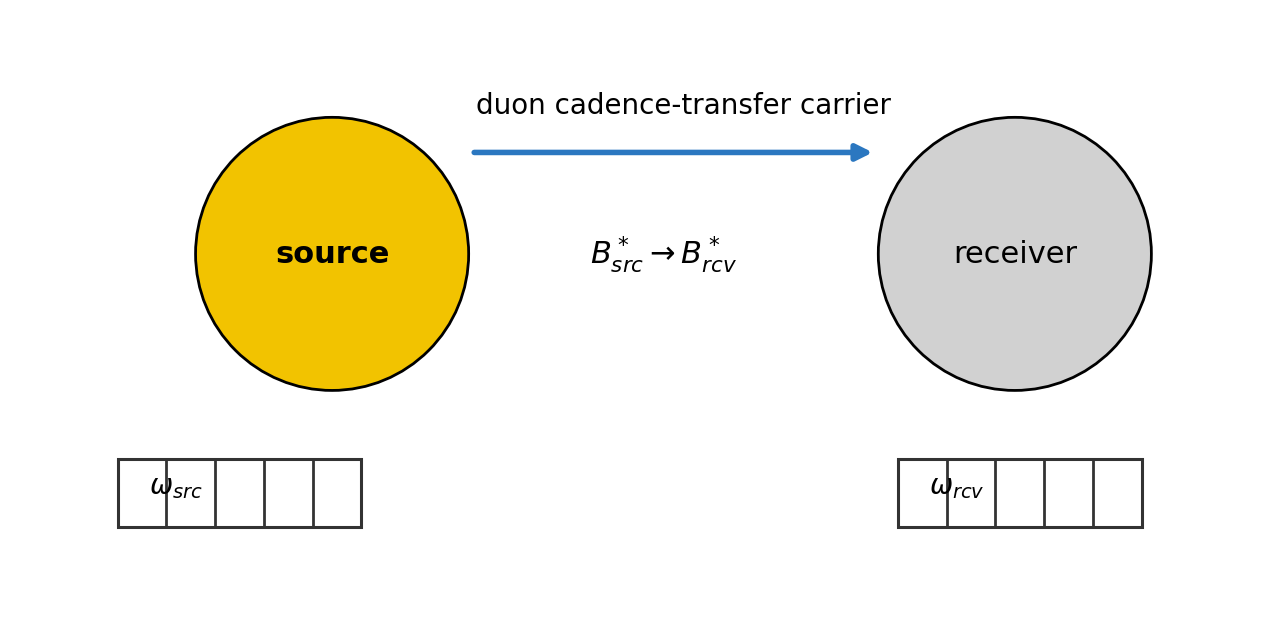
\includegraphics[width=0.78\linewidth]{figures/solar/redshift_duon_transfer.png}
\caption{Two-window duon cadence-transfer schematic. The source/receiver row is fixed first; the rendered solar redshift is attached afterward.}
\end{figure}

\paragraph{Hook / Evidence.} Use the cadence-transfer and two-window comparison hooks together with the duon-radiation bridge in the main note.

\paragraph{Companion notebook and manifest.} See Section~\ref{app:suppc-notebooks} for the executed calculation manifest and generated figure provenance for this section.

\begin{quote}\small\path{notebooks/solar/c2_c3_solar_radiation_worked.ipynb}\end{quote}
